\documentclass{article}
\usepackage[utf8]{inputenc}
\usepackage[newfloat]{minted}
\usepackage{graphicx}
\usepackage[capitalize, noabbrev]{cleveref}
\usepackage{caption}
\usepackage[section]{placeins}
\usepackage{fancyhdr}


\addtolength{\headheight}{1.5cm} % make more space for the header
\pagestyle{fancyplain} % use fancy for all pages except chapter start
\lhead{
\includegraphics[height=1.3cm]{logo_IT.png}} % left logo
%\lhead{\ }
%\rhead{
\includegraphics[height=1.5cm]{Figures/logo_IT.png}} % right logo
\rhead{\ }
\renewcommand{\headrulewidth}{0pt} % remove rule below header



\usemintedstyle{friendly}

\title{\textbf{360$^\circ$ Video Coding} \textbf{Simulation Tool}}
\author{João Carreira, José Filipe, António Navarro, Pedro Assunção}
\date{\today}

\begin{document}

\maketitle
\tableofcontents

%\newpage
\section{Overview of the graphical user interface}

\begin{figure}[ht]
    \centering
    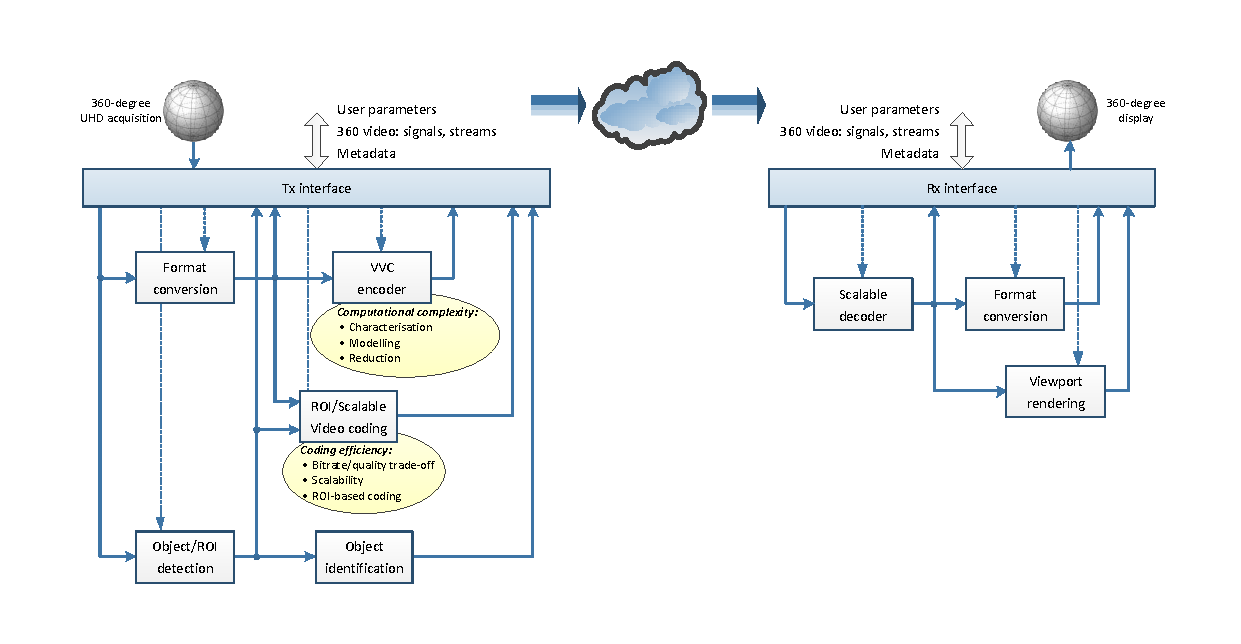
\includegraphics[width=1\textwidth]{ARoundVision_Framework_Diagram_v2.pdf}
    \caption{Tools and algorithms addressed in the ARoundVision project.}
    \label{fig:scheme}
\end{figure}

This section describes the high-level graphical user interface (GUI) which will allow to control the tools and algorithms developed in the ARoundVision project. \cref{fig:scheme} shows the overall diagram of this project. Mainly it can be divided into a transmitter ($T_x$) and a receiver ($R_x$). While the former is responsible for acquisition, pre-processing and data encoding, the latter is responsible for decoding, post-processing and display.

Our proposal is for a GUI to include both the $T_x$ and $R_x$ functions which can be split into different modules. The overall look of the GUI is depicted in \cref{fig:overall_gui}. The GUI is divided into two parts: Module selection and module interface. Each module is characterised by a different graphical interface which is drawn on the right and can include one or more functions. Each module is independent from each other, reducing the code complexity and allowing for extension in the future.

\begin{figure}[ht]
    \centering
    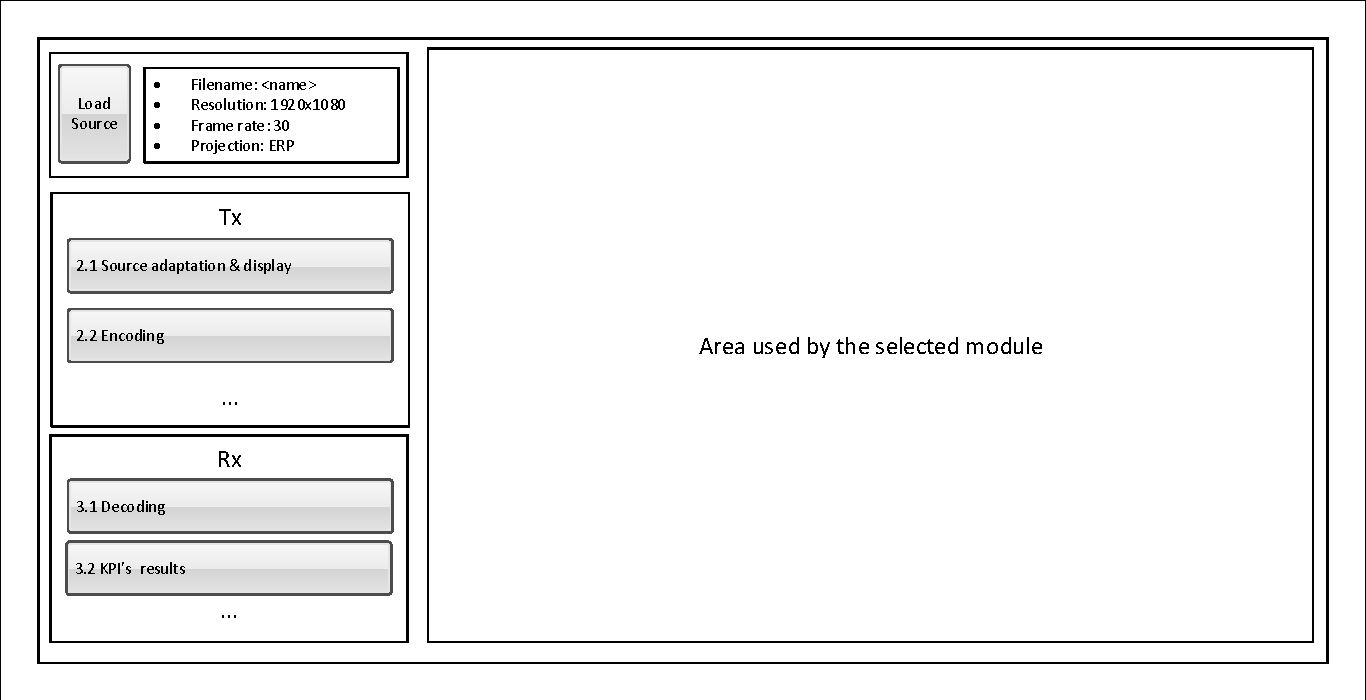
\includegraphics[page=1,width=1\textwidth]{Drawings.pdf}
    \caption{Overall aspect of our proposed GUI.}
    \label{fig:overall_gui}
\end{figure}

On the left the user is able to select the input source, which can either be an uncompressed video source or a compressed one, and next to the input selection, the video information is shown (resolution, frame rate, projection format, etc). Then, after a separator, a button for each module is shown allowing the user to select the desired module. Below the list of modules is described.

In order to select the input source, the created API returns a list of available sources, using the \mintinline{python}{Get360StreamList} function. Based on this the user can select an input using the \mintinline{python}{Select360Stream}. From this point on, all operation are applying to the selected stream.

% In order to select the input source, one can use a text-based file as shown in \cref{fig:results_module} with the information required, removing the need for extra dialog boxes to input extra information.
% This would be a generic format which can work for both raw/uncompressed and compressed video.
% While the former is meant for the $T_x$ modules, the latter is meant for the $R_x$ modules.

% \begin{figure}[htbp]
% \begin{minipage}[]{\linewidth}
% \begin{minted}[frame=single]{c}
% # Raw/Uncompressed source
% - source:
%   type: raw_video
%   filename: input.yuv
%   width: 3840
%   height: 1920
%   frame_rate: 30
%   frame_number: 100
%   pixel_format: YUV420p
%   projection: erp

% # or
% - source:
%   type: mkv
%   filename: input.mkv
%   ...

% # Compressed source
% - bitstream:
%   type: vvc_stream
%   filename: input.bin
%   ...
% \end{minted}
% \caption{Example of the configuration of input source in YAML format.}
% \label{cod:yml_enc_example}
% \end{minipage}
% \end{figure}

\section{$T_x$ Modules description}

This section describes the modules that theoretically belong to the transmitter ($T_x$) side.

\subsection{Display and adaptation}

This module is used to display the input 360$^\circ$ video, either from an uncompressed stream or from a capturing device.
The following functionality should be supported, according to \cref{fig:display_module}:

\begin{enumerate}
    \item Widget with support for zoom and pan operation, as well as, point and area selection. Use Use \mintinline{python}{GetFrame} to obtain a frame to display.

    \item  After selecting a fixed region-of-interest (ROI) in the widget with the 360-degree video, export to a file:
    \begin{enumerate}
        %\item Input source - this includes all information of source (see \cref{cod:yml_enc_example});
        \item Position;
        \item Size;
        %\item Frame number.
    \end{enumerate}

    \item Select between fixed and dynamic ROI (dynamic ROI implements object tracking, using existing tools). Use \mintinline{python}{GetFrame} with the desired projection.

    \item Open a window to select the destination projection and call the projection conversion function.

    \item Call the viewport rendering function with the selected ROI as input. Use \mintinline{python}{GetViewport} with the center and viewport dimensions obtained based on the selected ROI.

\end{enumerate}

\begin{figure}[htbp]
    \centering
    \includegraphics[page=2,width=1\textwidth]{Drawings.pdf}
    \caption{Display module.}
    \label{fig:display_module}
\end{figure}


% The first block detects object from an input 360-degree video signal. Each object is represented by a different region-of-interest highlighted in the video signal. Alternatively, they can be represented as different file formats.

% % \begin{figure}[htbp]
% %     \centering
% %     \includegraphics[page=4,width=0.65\textwidth]{Figures/results_file_example.png}
% %     \caption{Example of a results file (each column corresponds to a different result).}
% %     \label{fig:3}
% % \end{figure}

% The second step is to identify the detected objects. This block can receive a single output of the block represented in \cref{fig:scheme} and retrieve information regarding the object as metadata.

% % \begin{figure}[htbp]
% %     \centering
% %     \includegraphics[page=4,width=0.65\textwidth]{Figures/results_file_example.png}
% %     \caption{Example of a results file (each column corresponds to a different result).}
% %     \label{fig:3}
% % \end{figure}

% Based on these two blocks a graphical user interface could be constructed to show the object information as shown in the figure below.


\subsection{Encoding}

This module is used to encode the input source using different algorithms. This interface shall provide the following functionality according to \cref{fig:encoding_module}:

\begin{enumerate}
    \item Load selected options from file;

    \item Save selected options to a file;

    \item Call encoding function;

    \item Dynamic list of check boxes which are defined in a text file (see \cref{cod:encoding_options}).
\end{enumerate}

\begin{figure}[htbp]
    \centering
    \includegraphics[page=3,width=1\textwidth]{Drawings.pdf}
    \caption{Encoding module.}
    \label{fig:encoding_module}
\end{figure}

% \begin{figure}[htbp]
% \begin{minipage}[]{\linewidth}
% \begin{minted}[frame=single]{c}
% - encoding_module:
%   qp_list:
%     - 22
%     - 27
%     - 32
%     - 37

%   checkbox_list:
%     - complexity_reduction_algorithm_A
%     - complexity_reduction_algorithm_B
%     - complexity_reduction_algorithm_C
%     - spatial_scalability_algorithm_A
%     - spatial_scalability_algorithm_B
%     - spatial_scalability_algorithm_C
%     ...
% \end{minted}
% \end{minipage}
% \caption{Example of YAML file, defining the options shown in the encoding user interface.}
% \label{cod:encoding_options}
% \end{figure}

% \cref{cod:encoding_options} shows an example of a file listing the options to be displayed in the graphical user interface. For instance, a dropdown menu should allow the user to chose a QP value, form the options $22$, $27$, $32$ and $37$. Furthermore, the checkbox list presents the options available to the user that can be selected by ticking the checkboxes.

% In turn, \cref{cod:options_selected} shows the options mentioned above, that were selected by the user. This file serves two purposes: persisting the configurations set through the GUI for the encoder, when the `Save Config' button is hit, and serving as an interface between the GUI and the encoder when the `Encode' button is hit.

% \begin{figure}[htbp]
% \begin{minipage}[]{\linewidth}
% \begin{minted}[frame=single]{c}
% - encoding_options:
%   cfg_files_paths_list:
%     - "/cfg/encoder_randomaccess_vtm.cfg"
%     - "/cfg-360Lib/per-sequence/360/360test_Harbor.cfg"
%     - "/cfg-360Lib/encoder_360_ERP.cfg"

%   qp:
%     - 22

%   rate_control:
%     - 50000

%   number_of_frames_to_encode:
%     - 10

%   ticked_checkboxes:
%     - complexity_reduction_algorithm_A
%     - spatial_scalability_algorithm_C
% \end{minted}
% \end{minipage}
% \caption{Example of YAML configuration for the encoding module.}
% \label{cod:options_selected}
% \end{figure}

When the user presses the "Add" button, a user interface showing the configuration files obtained with the \mintinline{latex}{GetCfgFiles} should be shown. Then the user can add the desired configuration files one by one. The selected files should be show in the list of encoder config files. The "Remove" button should allow the user to remove a button from this list. Then, the user should choose one of the QPs from the dropdown. The options available form the dropdown are given by \mintinline{latex}{GetQPs}. The user should not set all the desired parameters using the interface. When the user presses the "Encode" button, two functions will be called. First, the \mintinline{latex}{SetEncodingParams} function will read all the fields set by the user in the user interface and pass them to the class that manages the encoding process. Then the \mintinline{latex}{LaunchEncodingProcess} function is launched, triggering the beginning of the encoding process itself. Note that "Load Config" and "Save Config" buttons should allow the user to save and load respectively the values introduced in the user interface, in order to have reproducible experiments.


\section{$R_x$ Modules description}

This section describes the modules that theoretically belong to the receiver ($R_x$) side.


\subsection{Decoding}

This module is responsible for decoding a previously compressed bitstream. This user interface should integrate the following functionalities, according with \cref{fig:encoding_module}:

\begin{enumerate}
    \item Video player, showing the decoded sequence.
    \item Panel containing information about the bitstream. If a scalable version of the encoder was used to encode the bitstream, informations of the various layer should be displays, such as the number of layers for instance.
    \item Drop-down menu with decoder options. For instance this menu should allow the user to enable or disable the Decoder Side Motion Vector Refinement tool, or in case of scalable video, select witch layer should be decoded.
\end{enumerate}

\begin{figure}[h!]
    \centering
    \includegraphics[page=5,width=1\textwidth]{Drawings.pdf}
    \caption{Decoding module.}
    \label{fig:decoding_module}
\end{figure}

\subsection{Key Performance Indicators}

This module should allow the user to analyse and compare the results of the performance of several encoded sequences. It should be possible to trace Rate-Distortion (RD) curves, using this module. However, the module should give more flexibility to the user, allowing him to chose the values to be shown in the $x$ and $y$ axis. For this purpose, the Key Performance Indicators (KPI) module should include the following functionalities, according with \cref{fig:results_module}:

\begin{enumerate}
    \item Button for adding a file containing the performance results of a given encoded sequence, containing metrics such as PSNR, Bitrate, etc. A button for removing an already loaded file should also be present.
    \item A list, showing the files already loaded.
    \item A dropdown menu, that allows the user to choose which of the metrics present in the files loaded through 1. should be displayed in the $x$ axis. The options present in this menu should be dynamically inferred form the values present in the loaded files. This can be done based on the first row of the results file.
    \item A similar dropdown menu, that allows the user to choose the values to be shown in the $y$ axis. The options should also be inferred from the values present in the loaded files.
    \item A panel displaying the $y(x)$ plot, defined by the dropdown menus. Extra toggles can be present to change the plot configuration, such as, changing between lines and bars, or control the axis range.
\end{enumerate}

\begin{figure}[htbp]
    \centering
    \includegraphics[page=4,width=1\textwidth]{Drawings.pdf}
    \caption{Results analysis module.}
    \label{fig:results_module}
\end{figure}

\begin{figure}[htbp]
    \centering
    \includegraphics[width=1\textwidth]{results_file_example.png}
    \caption{Example of a results file (each column corresponds to a different result).}
    \label{fig:results_file_example}
\end{figure}

\cref{fig:results_file_example} shows an example of how the file containing the results of the compression process should look like.


\section{API Documentation}

In order to allow for the functionalities described above API will be defined including one or more \textit{classes} which will allow for:
\begin{enumerate}
    \item read/capture 360$^\circ$ video;
    \item process and return the video stream frame by frame to the GUI;
    \item format conversion;
    \item encode the video stream;
    %\item decode existing 360$^\circ$ stream previously encoded.
\end{enumerate}

This API is available at \textit{https://gitlab.com/aroundvision/arvapy} (private repository). The implementation can be run using a docker container (discuss how should we share it).


\subsection{Display and adaptation}

%%%%%%%%%%%%%%%%%%%%%%%%%%%%%%%%%%%%%%%%%%%%%%%%%%%%%%%%%%%%%%%%%%%%%%%%%%%%%%%%%%%%%%%%%%%%%%%%%%%%%%%%

\subsubsection*{\mintinline{python}{Get360StreamList}}

This function returns a list of arrays with the following information in order: name, width, height, bytes per pixel.

\textbf{Returns}

\mintinline{latex}{JSON object}: list of arrays (one for each sequence)

\textbf{Route}

\mintinline{python}{host/get_stream_list}

%%%%%%%%%%%%%%%%%%%%%%%%%%%%%%%%%%%%%%%%%%%%%%%%%%%%%%%%%%%%%%%%%%%%%%%%%%%%%%%%%%%%%%%%%%%%%%%%%%%%%%%%

\subsubsection*{\mintinline{python}{GetLayerInfo}}

This function returns the information regarding the available layer of a given stream.

\textbf{Returns}

\mintinline{latex}{JSON object}: list of pairs (layer idx, layer description)

\textbf{Route}

\mintinline{python}{host/get_layer_info}


%%%%%%%%%%%%%%%%%%%%%%%%%%%%%%%%%%%%%%%%%%%%%%%%%%%%%%%%%%%%%%%%%%%%%%%%%%%%%%%%%%%%%%%%%%%%%%%%%%%%%%%%

\subsubsection*{\mintinline{python}{Select360Stream}}

This function selects the desired 360-degree stream.

\textbf{Arguments}

\mintinline{latex}{int idx}: index of the video stream in the array returned by \mintinline{python}{Get360StreamList}

\textbf{Returns}

\mintinline{latex}{Bool}: True if succeeded (False otherwise)

\textbf{Route}

\mintinline{python}{host/select_stream}

%%%%%%%%%%%%%%%%%%%%%%%%%%%%%%%%%%%%%%%%%%%%%%%%%%%%%%%%%%%%%%%%%%%%%%%%%%%%%%%%%%%%%%%%%%%%%%%%%%%%%%%%

\subsubsection*{\mintinline{python}{GetProjectionList}}

This function returns the list of available planar projection formats

\textbf{Returns}

\mintinline{latex}{JSON object}: list with pairs of projection initial and name

\textbf{Route}

\mintinline{python}{host/get_projections}


%%%%%%%%%%%%%%%%%%%%%%%%%%%%%%%%%%%%%%%%%%%%%%%%%%%%%%%%%%%%%%%%%%%%%%%%%%%%%%%%%%%%%%%%%%%%%%%%%%%%%%%%

\subsubsection*{\mintinline{python}{GetFrameInfo}}

This function returns the information regarding a frame

\textbf{Arguments}

\mintinline{latex}{string projection}: initials of the planar projection format of the output (default means original projection)
\mintinline{latex}{int layer}: layer to return (default means highest layer)

\textbf{Returns}

\mintinline{latex}{JSON object}:  width, height and bytes/pixel of the frame in a given projection.

\textbf{Route}

\mintinline{python}{host/get_frame_info}

%%%%%%%%%%%%%%%%%%%%%%%%%%%%%%%%%%%%%%%%%%%%%%%%%%%%%%%%%%%%%%%%%%%%%%%%%%%%%%%%%%%%%%%%%%%%%%%%%%%%%%%%

\subsubsection*{\mintinline{python}{GetFrameRaw}}

This function returns a new raw frame (no signalling) on every call

\textbf{Arguments}

\mintinline{latex}{string projection}: initials of the planar projection format of the output (default means original projection)
\mintinline{latex}{int layer}: layer to return (default means highest layer)

\textbf{Returns}

\mintinline{latex}{Byte array}: new frame in raw format

\textbf{Route}

\mintinline{python}{host/get_frame_raw}

%%%%%%%%%%%%%%%%%%%%%%%%%%%%%%%%%%%%%%%%%%%%%%%%%%%%%%%%%%%%%%%%%%%%%%%%%%%%%%%%%%%%%%%%%%%%%%%%%%%%%%%%

\subsubsection*{\mintinline{python}{GetFrame}}

This function returns a new frame on every call.
At the beginning of the byte stream a sequence of ASCII:
\begin{verbatim}
[width]x[height]\n
[bytes per pixel (Bpp)]\n
( width * height * Bpp ) pixels bytes
\end{verbatim}

\textbf{Arguments}

\mintinline{latex}{string projection}: initials of the planar projection format of the output (default means original projection)
\mintinline{latex}{int layer}: layer to return (default means highest layer)

\textbf{Returns}

\mintinline{latex}{Byte array}: header + bytes of the frame

\textbf{Route}

\mintinline{python}{host/get_frame}

%%%%%%%%%%%%%%%%%%%%%%%%%%%%%%%%%%%%%%%%%%%%%%%%%%%%%%%%%%%%%%%%%%%%%%%%%%%%%%%%%%%%%%%%%%%%%%%%%%%%%%%%

\subsubsection*{\mintinline{python}{GetProejctionFaceInfo}}

This function returns part of the 360-degree video frame.
For example it returns a face of a polyhedron-based projection.

Currently, it will always return a face of the cube-map projection.
In future it will return a frame from each projection selected.

\textbf{Arguments}

\mintinline{latex}{string projection}: initials of the planar projection format of the output (default means original projection)
\mintinline{latex}{int face}: the number of the face
\mintinline{latex}{int layer}: layer to return (default means highest layer)

\textbf{Returns}

\mintinline{latex}{JSON object}:  width, height and bytes/pixel of the frame containingthe a face of a given projection.

\textbf{Route}

\mintinline{python}{host/get_projection_face_info}

%%%%%%%%%%%%%%%%%%%%%%%%%%%%%%%%%%%%%%%%%%%%%%%%%%%%%%%%%%%%%%%%%%%%%%%%%%%%%%%%%%%%%%%%%%%%%%%%%%%%%%%%

\subsubsection*{\mintinline{python}{GetProjectionFaceRaW}}

This function returns part of the 360-degree video frame.
For example it returns a face of a polyhedron-based projection in raw format (no signalling) on every call.

Currently, it will always return a face of the cube-map projection.
In future it will return a frame from each projection selected.

\textbf{Arguments}

\mintinline{latex}{string projection}: initials of the planar projection format of the output (default means original projection)
\mintinline{latex}{int face}: the number of the face
\mintinline{latex}{int layer}: layer to return (default means highest layer)

\textbf{Returns}

\mintinline{latex}{Byte array}: new frame in raw format

\textbf{Route}

\mintinline{python}{host/get_projection_face_raw}

%%%%%%%%%%%%%%%%%%%%%%%%%%%%%%%%%%%%%%%%%%%%%%%%%%%%%%%%%%%%%%%%%%%%%%%%%%%%%%%%%%%%%%%%%%%%%%%%%%%%%%%%

\subsubsection*{\mintinline{python}{GetProjectionFace}}

This function returns part of the 360-degree video frame on every call (with signalling).
At the beginning of the byte stream a sequence of ASCII:
\begin{verbatim}
[width]x[height]\n
[bytes per pixel (Bpp)]\n
( width * height * Bpp ) pixels bytes
\end{verbatim}

\textbf{Arguments}

\mintinline{latex}{string projection}: initials of the planar projection format of the output (default means original projection)
\mintinline{latex}{int face}: the number of the face
\mintinline{latex}{int layer}: layer to return (default means highest layer)

\textbf{Returns}

\mintinline{latex}{Byte array}:  header + bytes of the face requested

\textbf{Route}

\mintinline{python}{host/get_projection_face}

%%%%%%%%%%%%%%%%%%%%%%%%%%%%%%%%%%%%%%%%%%%%%%%%%%%%%%%%%%%%%%%%%%%%%%%%%%%%%%%%%%%%%%%%%%%%%%%%%%%%%%%%

\subsubsection*{\mintinline{python}{GetViewportInfo}}

This function returns a viewport of the current frame

\textbf{Arguments}

\mintinline{latex}{string coord}: coordinate system (pixel, polar)

\mintinline{latex}{int x}: viewport horizontal center position in degrees

\mintinline{latex}{int y}: viewport vertical center position in degrees

\mintinline{latex}{int width}: width of the viewport in degree

\mintinline{latex}{int height}: height of the viewport in degrees

\mintinline{latex}{int layer}: layer to return (default means highest layer)

\textbf{Returns}

\mintinline{latex}{JSON object}: width, height and bytes/pixel of the viewport frame.

\textbf{Route}

\mintinline{python}{host/get_viewport_info}

%%%%%%%%%%%%%%%%%%%%%%%%%%%%%%%%%%%%%%%%%%%%%%%%%%%%%%%%%%%%%%%%%%%%%%%%%%%%%%%%%%%%%%%%%%%%%%%%%%%%%%%

\subsubsection*{\mintinline{python}{GetViewportRaw}}

This function returns a new frame with the desired viewport on every call.
At the beginning of the byte stream a sequence of ASCII:
\begin{verbatim}
[width]x[height]\n
[bytes per pixel (Bpp)]\n
( width * height * Bpp ) pixels bytes
\end{verbatim}

\textbf{Arguments}

\mintinline{latex}{string coord}: coordinate system (pixel, polar)

\mintinline{latex}{int x}: viewport horizontal center position in degrees

\mintinline{latex}{int y}: viewport vertical center position in degrees

\mintinline{latex}{int width}: width of the viewport in degree

\mintinline{latex}{int height}: height of the viewport in degrees

\mintinline{latex}{int layer}: layer to return (default means highest layer)

\textbf{Returns}

\mintinline{latex}{Byte array}: header + byte array of the generated viewport

\textbf{Route}

\mintinline{python}{host/get_viewport_raw}

%%%%%%%%%%%%%%%%%%%%%%%%%%%%%%%%%%%%%%%%%%%%%%%%%%%%%%%%%%%%%%%%%%%%%%%%%%%%%%%%%%%%%%%%%%%%%%%%%%%%%%%

\subsubsection*{\mintinline{python}{GetViewport}}

This function returns a new frame with the desired viewport on every call.
At the beginning of the byte stream a sequence of ASCII:
\begin{verbatim}
[width]x[height]\n
[bytes per pixel (Bpp)]\n
( width * height * Bpp ) pixels bytes
\end{verbatim}

\textbf{Arguments}

\mintinline{latex}{string coord}: coordinate system (pixel, polar)

\mintinline{latex}{int x}: viewport horizontal center position in degrees

\mintinline{latex}{int y}: viewport vertical center position in degrees

\mintinline{latex}{int width}: width of the viewport in degree

\mintinline{latex}{int height}: height of the viewport in degrees

\mintinline{latex}{int layer}: layer to return (default means highest layer)

\textbf{Returns}

\mintinline{latex}{Byte array}: header + byte array of the generated viewport

\textbf{Route}

\mintinline{python}{host/get_viewport}




%%%%%%%%%%%%%%%%%%%%%%%%%%%%%%%%%%%%%%%%%%%%%%%%%%%%%%%%%%%%%%%%%%%%%%%%%%%%%%%%%%%%%%%%%%%%%%%%%%%%%%%%

\subsection{Encoding}

\subsubsection*{\mintinline{python}{GetCfgFiles}}

This function returns a list with the paths for all configuration (*.cfg) files found in the search path.

\textbf{Returns}

\mintinline{latex}{List object}: list of paths to all configuration files

\textbf{Route}

\mintinline{python}{host/get_cfg_paths}

%%%%%%%%%%%%%%%%%%%%%%%%%%%%%%%%%%%%%%%%%%%%%%%%%%%%%%%%%%%%%%%%%%%%%%%%%%%%%%%%%%%%%%%%%%%%%%%%%%%%%%%%

\subsubsection*{\mintinline{python}{GetCfgFiles}}

This function returns a list with the paths for all configuration (*.cfg) files found in the search path.

\textbf{Returns}

\mintinline{latex}{List object}: list of paths to all configuration files

\textbf{Link}

\mintinline{python}{host/get_cfg_paths}

%%%%%%%%%%%%%%%%%%%%%%%%%%%%%%%%%%%%%%%%%%%%%%%%%%%%%%%%%%%%%%%%%%%%%%%%%%%%%%%%%%%%%%%%%%%%%%%%%%%%%%%%

\subsubsection*{\mintinline{python}{GetQPs}}

This function returns the list of usable QP values

\textbf{Returns}

\mintinline{latex}{List object}: list with usable QPs

\textbf{Link}

\mintinline{python}{host/get_qps}

%%%%%%%%%%%%%%%%%%%%%%%%%%%%%%%%%%%%%%%%%%%%%%%%%%%%%%%%%%%%%%%%%%%%%%%%%%%%%%%%%%%%%%%%%%%%%%%%%%%%%%%%

\subsubsection*{\mintinline{python}{SetEncodingParams}}

This function sets the necessary parameters for generating a valid encoding command

\textbf{Arguments}

\mintinline{latex}{string orig_yuv_path}: path to the sequence to be encoded

\mintinline{latex}{string rec_yuv_pat}: path where the reconstructed sequence after enconding is to be stored

\mintinline{latex}{string out_bin_path}: path where the compressed sequence is to be stored

\mintinline{latex}{list cfg_files}: list of strings containing the paths for the cofiguration files (as given by GetCfgFiles) to be used

\mintinline{latex}{list qp}: list of integers, containing the QP values to be used

\textbf{Route}

\mintinline{python}{host/set_encoder_params}

%%%%%%%%%%%%%%%%%%%%%%%%%%%%%%%%%%%%%%%%%%%%%%%%%%%%%%%%%%%%%%%%%%%%%%%%%%%%%%%%%%%%%%%%%%%%%%%%%%%%%%%%

\subsubsection*{\mintinline{python}{LaunchEncodingProcess}}

This function lauches the encoding precesses defined by SetEncodingParams

\textbf{Route}

\mintinline{python}{host/lauch_enc_proc}

%%%%%%%%%%%%%%%%%%%%%%%%%%%%%%%%%%%%%%%%%%%%%%%%%%%%%%%%%%%%%%%%%%%%%%%%%%%%%%%%%%%%%%%%%%%%%%%%%%%%%%%%

\end{document}
